% !TeX root = ../dokumentation.tex

\chapter{Sprints} \label{sprints}

\section{Sprint 1}
\todo{Beschreibung des Produktincrements}

\section{Ziele Sprint 1}
\todo{Ziel Sprint 1}

\section{Ergebnisse Sprint 1}

\subsection{Produktincrement}
\subsection{Charts}

\subsection{Probleme und Verbesserungen}
\todo{Retro Ergebnisse}


\subsection{Bearbeitete User Storys}
\subsubsection{SKIOS-22 POC for keycloak}
Das Ticket \enquote{SKIOS-22 POC for keycloak} hatte folgende User Story:
\begin{quotation}
    As a developer I would like to have a POC for two services using keycloak~\parencite{web/Keycloak} so that I`ll know how users will be managed in the future. \\
    \textbf{Acceptance Criteria}
    \begin{itemize}
        \item A backend service has an api that can get information about the logged in user
        \item A frontend service can create users (in any primitive way) and log in + send a request to the aformentioned endpoint
        \item Our keycloak~\parencite{git/skiosa/orm} instance is configured to work with both services
    \end{itemize}
\end{quotation}
Bearbeitet von Tim Horlacher.
Reviewed von Lukas Huida.

\subsubsection{SKIOS-29 Undesigned Angular Boilerplate}
Das Ticket \enquote{SKIOS-29 Undesigned Angular Boilerplate} hatte folgende User Story:
\begin{quotation}
    As a developer I would like a boilerplate for angular to be created so that I can start work on the project. \\
    \textbf{Acceptance Criteria}
    \begin{itemize}
        \item An angular boilderplate exists with basic pages and routing
        \item A central structure for requests (using services) is created
        \item Infrastructure for passing global data (such as a username) is implemented
    \end{itemize}
\end{quotation}
Bearbeitet von Tim Horlacher.
Reviewed von Lukas Huida.

\subsubsection{SKIOS-31 Evaluate Core-Service}
Das Ticket \enquote{SKIOS-31 Evaluate Core-Service} hatte folgende User Story:
\begin{quotation}
    As a developer I would like to know which ORM will be used and whether or not to base our APIs around GraphQL~\parencite{web/GraphQL} or to stick with REST within the Core service. \\
    \textbf{Acceptance Criteria}
    \begin{itemize}
        \item It is clear, what ORM to use and is documented somewhere (ex. comments of this story)
        \item It is clear if GraphQL~\parencite{web/GraphQL} is used and findings are documented somewhere aswell
    \end{itemize}
\end{quotation}
Bearbeitet von Tim Horlacher.
Reviewed von Lukas Huida.

\subsubsection{SKIOS-32 Preliminary Polling service}
Das Ticket \enquote{SKIOS-32 Preliminary Polling service} hatte folgende User Story:
\begin{quotation}
    As a developer I would like a basic boilerplate for the polling service so that development can start.
    Functionally this Polling service only loads mock data into the database (intervall will be implemnted in k8s and not here) and isn't a \enquote{basic polling service}.
\textbf{Acceptance Criteria}
\begin{itemize}
    \item Mock data is loaded into the database at startup
    \item Basic boilerplate and infrastructure for the service is created (ex. project and file/directory structure)
    \item Mock data isn't provided from an RSS feed 
    \item Basic testing framework is set up
\end{itemize}
\end{quotation}
Bearbeitet von Jannik Springer.
Reviewed von Lukas Huida.

\subsubsection{SKIOS-34 List of Participants}
Das Ticket \enquote{SKIOS-34 List of Participants} hatte folgende User Story:
\begin{quotation}
    As our lecturer I would like a list of group members so that I can grade the project. \\
    \textbf{Acceptance Criteria}
    \begin{itemize}
        \item A list is created including all 11 names and matnr.
        \item Said list is given to the professor
    \end{itemize}
\end{quotation}
Bearbeitet von Tim Horlacher.
Reviewed von Lukas Huida.

\subsubsection{SKIOS-52 Devcontainer Guide}
Das Ticket \enquote{SKIOS-52 Devcontainer Guide} hatte folgende User Story:
\begin{quotation}
    As a developer I would like a guide on the usage of devcontainers for development. \\
    \textbf{Acceptance Criteria}
    \begin{itemize}
        \item A guide is created in confluence
        \item A sample devcontainer is implemented
        \item Other developers are taught about devcontainers 
    \end{itemize}
\end{quotation}
Bearbeitet von Tim Horlacher.
Reviewed von Lukas Huida.

\subsubsection{SKIOS-13 Create Basic Infrastructure}
Das Ticket \enquote{SKIOS-13 Create Basic Infrastructure} hatte folgende User Story:
\begin{quotation}
    Als Product Owner möchte ich die Möglichkeit haben das unser Produkt weltweit sicher erreichbar ist. Um das zu erreichen, muss ein Server mit einer passenden gemietet werden. \\
    \textbf{Acceptance Criteria}
    \begin{itemize}
        \item Die Domain \enquote{Skiosa.de} bestellt und dem Server zugewiesen.
        \item Einen passenden Server bestellt und mit notwendigen Tools wie SSH aufgesetzt.
        \item K3S Basis Installation.
        \item kubectl von Remote erreichbar und eingerichtet.
        \item Firewall Regeln angelegt um nur Web, SSH und Kubectl zuzulassen.
    \end{itemize} 
\end{quotation}
Bearbeitet von Lukas Huida.
Reviewed von Tim Horlacher.

\subsubsection{SKIOS-18 Basic Kubernetes Infra}
Das Ticket \enquote{SKIOS-18 Basic Kubernetes Infra} hatte folgende User Story:
\begin{quotation}
    As a infra member I want a basic Infrastructure based on Kubernetes. This Infrastructure should container some CI/CD pipeline software and examples to implement
    a CI/CD pipeline for our services. \\
    \textbf{Acceptance Criteria}
    \begin{itemize}
        \item Working Ingress-Controller with correct Certs
        \item Self-Hosted Docker-Registry
        \item ArgoCD Setup
        \item Drone.io Setup
        \item SonarQube Setup
        \item Keycloak Setup
        \item HashiCorp Vault Setup (Optional)
    \end{itemize}
\end{quotation}
Bearbeitet von Lukas Huida.
Reviewed von Tim Horlacher.

\subsubsection{SKIOS-9 Create Continous Integration Pipeline}
Das Ticket \enquote{SKIOS-9 Create Continuos Integration Pipeline} hatte folgende User Story:
\begin{quotation}
    As a developer I want my code to be tested and analyzed by sonar after every new commit so that our platform can ensure stability. \\
    \textbf{Acceptance Criteria}
    \begin{itemize}
        \item A pipeline exists for every service.
        \item A commit pipeline is triggered after every commit on a non master branch. This pipeline runs through: unit tests and sonarqube.
        \item A pr pipeline is triggered after a pull requests is created. This pipeline runs through: unit tests, integration tests and sonarqube.
        \item A main pipeline is triggered after a merge of a master branch. This pipeline runs through: unit tests, container build, CD-Script and sonarqube.
    \end{itemize}
\end{quotation}
Bearbeitet von Lukas Huida.
Reviewed von Tim Horlacher.

\subsubsection{SKIOS-10 Create Continous Delivery Pipeline}
Das Ticket \enquote{SKIOS-10 Create Continuos Delivery Pipeline} hatte folgende User Story:
\begin{quotation}
    As a developer I want my code to be delivered to prod after I merge it to master. \\
    \textbf{Acceptance Criteria}
    \begin{itemize}
        \item pipeline is triggered after merge to master
        \item pipeline tests code with unit/sonar before merge (is already managed by ci-pipeline)
        \item pipeline tests code with newman after merge → fail leads to rollback
    \end{itemize}
\end{quotation}
Bearbeitet von Lukas Huida.
Reviewed von Jonas Eppard.

\subsubsection{SKIOS-21 Initialize Keycloak}
Das Ticket \enquote{SKIOS-21 Initialize Keycloak} hatte folgende User Story:
\begin{quotation}
    As a developer I would like to have Keycloak setup so that we can test its usefulness. \\
    \textbf{Acceptance Criteria}
    \begin{itemize}
        \item A Keycloak server is running in our cluster and is reachable.
    \end{itemize}
\end{quotation}
Bearbeitet von Lukas Huida.
Reviewed von Tim Horlacher.

\subsubsection{SKIOS-30 Preliminary Core service}
Das Ticket \enquote{SKIOS-30 Preliminary Core service} hatte folgende User Story:
\begin{quotation}
    As a developer I want to have a basic core service with some boilerplate and mock endpoints to get started in the frontend. \\
    \textbf{Acceptance Criteria}
    \begin{itemize}
        \item be able to fetch mock articles with graphql
    \end{itemize}
\end{quotation}
Bearbeitet von Lukas Huida.
Reviewed von Tim Horlacher.

\subsubsection{SKIOS-37 Decision of Programming Database}
Das Ticket \enquote{SKIOS-37 Decision of Programming Database} hatte folgende User Story:
\begin{quotation}
    As a developer I need to know which database is used, to know which database connector for ORMs are needed. \\
    \textbf{Acceptance Criteria}
    \begin{itemize}
        \item A decision of a database is done
        \item The decision is documented in Confluence
    \end{itemize}
\end{quotation}
Bearbeitet von Lukas Huida.
Reviewed von Jonas Eppard.

\subsubsection{SKIOS-38 Contribution Guidelines}
Das Ticket \enquote{SKIOS-38 Contribution Guidelines} hatte folgende User Story:
\begin{quotation}
    As a developer I would like to have a guidline for making contributions so that we have a defined process to get code resulting from stories into production. \\
\textbf{Acceptance Criteria}
\begin{itemize}
    \item Contribution Guidlines are documented in Confluence
    \item Git Guidelines for naming schemes for git commits, branch names etc., squash/rebase merging are documented
    \item Review and Testing has a process, defining what should be reviewed (integration tests, code style, etc) and who should review it
    \item Code comments and code styles are defined and agreed upon by every member
    \item Documentation style, including what to document where (Confluence vs. Git) is clarified
    \item It is clarified when a task counts as done (review of dev, review of po, dev and tech lead, only review of tech/service lead)
\end{itemize}
\end{quotation}
Bearbeitet von Simon Morgenstern.
Reviewed von Amos Groß.

\subsubsection{SKIOS-39 Guidelines Testing}
Das Ticket \enquote{SKIOS-39 Guidelines Testing} hatte folgende User Story:
\begin{quotation}
    As a developer I would like to have a guideline for testing so that I can know if I'm testing my code correctly. \\
\textbf{Acceptance Criteria}
\begin{itemize}
    \item The types of tests are clarified (unit, integration, manual, cypress/selenium, etc.)
    \item The amount of test that have to be written is clear (ex. test coverage, integration test for ever use case or error, etc)
    \item A decision is made when, where and by whom tests have to be written (ex. in separate stories per epic, implicitly with every story, etc.)
    \item All findings are documented in confluence
\end{itemize}
\end{quotation}
Bearbeitet von Simon Morgenstern.
Reviewed von Amos Groß.

\subsubsection{SKIOS-40 Testing Frameworks}
Das Ticket \enquote{SKIOS-40 Testing Frameworks} hatte folgende User Story:
\begin{quotation}
    As a developer, I would like to know which testing frameworks I need to use so that I can write tests. \\
\textbf{Acceptance Criteria}
\begin{itemize}
    \item Testing frameworks for every language are decided upon
    \item The testing frameworks are added to the services documentation in confluence
    \item Programs to to integration tests with are clear
\end{itemize}
\end{quotation}
Bearbeitet von Simon Morgenstern.
Reviewed von Amos Groß.

\subsubsection{SKIOS-49 Create Example Service}
Das Ticket \enquote{SKIOS-49 Create Example Service} hatte folgende User Story:
\begin{quotation}
    As a developer I want an example service to test the CI/CD pipeline. \\
    \textbf{Acceptance Criteria}
    \begin{itemize}
        \item An example service exists
        \item A example deployment is created
        \item A example CI pipeline is working with the example service
    \end{itemize}
\end{quotation}
Bearbeitet von Lukas Huida.
Reviewed von Tim Horlacher.

\subsubsection{SKIOS-50 Deploy Database}
Das Ticket \enquote{SKIOS-50 Deploy Database} hatte folgende User Story:
\begin{quotation}
    As a developer I want a central database to store my objects and articles. \\
    \textbf{Acceptance Criteria}
    \begin{itemize}
        \item PostgreSQL is deployed in a db namespace
        \item db is reachable in the default namespace with credentials stored at the vault
    \end{itemize}
\end{quotation}
Bearbeitet von Lukas Huida.
Reviewed von Jonas Eppard.

\subsubsection{SKIOS-64 Guideline for Issues}
Das Ticket \enquote{SKIOS-64 Guideline for Issues} hatte folgende User Story:
\begin{quotation}
    As a product owner, I would like to have a guideline for new issues so that the team can understand what their work is. \\
\textbf{Acceptance Criteria}
\begin{itemize}
    \item Issue Guideline is documented in confluence
    \item Structure for future stories is clear
\end{itemize}
\end{quotation}
Bearbeitet von Simon Morgenstern.
Reviewed von Amos Groß.

\subsubsection{SKIOS-11 Update Mockups for possible design language}
Das Ticket \enquote{SKIOS-11 Update Mockups for possible design language} hatte folgende User Story:
\begin{quotation}
    As a ui/ux designer, I would like to like to have a design language to follow when creating mockups.
    If you're unsure about what a design langage is, the following article explains it:  (this story references the \enquote{Style guidelines} part of their definition)
    Also interesting thing to look up might be UI/UX design in general to understand why design languages matter and are necessary for good software. \\
\textbf{Acceptance Criteria}
\begin{itemize}
    \item deas are documented in confluence
    \item Figma Mock ups now represent new design language
    \item Decisions on fonts, separation of pages and page structure are made
    \item A clear design language is implemented for Skiosa
\end{itemize}
\end{quotation}
Bearbeitet von Amos Groß.
Reviewed von Lukas Huida.

\subsubsection{SKIOS-27 Document Initial Requirements}
Das Ticket \enquote{SKIOS-27 Document Initial Requirements} hatte folgende User Story:
\begin{quotation}
    As a product owner I want the plattform's requirements and features to be documented, so that we can refer to it in the final documentation. \\
\textbf{Acceptance Criteria}
\begin{itemize}
    \item All Requirements are listed in a confluence page
    \item Must haves and optional requirements are listed or indicated as such
\end{itemize}
\end{quotation}
Bearbeitet von Amos Groß.
Reviewed von Lukas Huida.

\subsubsection{SKIOS-33 Mockups for Central Pages}
Das Ticket \enquote{SKIOS-33 Mockups for Central Pages} hatte folgende User Story:
\begin{quotation}
    As a developer I would like to have mockups of the main pages, so that it is clear how to design the frontend. \\
\textbf{Acceptance Criteria}
\begin{itemize}
    \item Mockups are created in figma
    \item Overview and View pages have mockups
    \item The Mockups have been discussed with the team (ie. review)
    \item Mockups contain desktop and mobile versions
\end{itemize}
\end{quotation}
Bearbeitet von Amos Groß.
Reviewed von Lukas Huida.

\subsubsection{SKIOS-43 Fix Jira Workflow}
Das Ticket \enquote{SKIOS-43 Fix Jira Workflow} hatte folgende User Story:
\begin{quotation}
    As a developer I want to see if a Issue/Story/Ticket is Done. At the moment if its done the story is not crossed out as at should be. \\ 
\textbf{Acceptance Criteria}
\begin{itemize}
    \item Tickets/Story/Issues are crosses out if there are done/resolved.
\end{itemize}
\end{quotation}
Bearbeitet von Amos Groß.
Reviewed von Lukas Huida.

\subsubsection{SKIOS-57 Figma Colors}
Das Ticket \enquote{SKIOS-57 Figma Colors} hatte folgende User Story:
\begin{quotation}
    As a ui/ux designer, I would like to have a central style in figma to base color choices off of.

    Subject of this story is to create a style based off of whatever the current color scheme is and to replace all instances of that color with the style. \\
\textbf{Acceptance Criteria}
\begin{itemize}
    \item A new style is created in the figma draft
    \item All hardcoded colors are replaced with mentions of styles
    \item The colors in the style have names (as explained above)
\end{itemize}
\end{quotation}
Bearbeitet von Marcel Alex.
Reviewed von Amos Groß.

\subsubsection{SKIOS-66 LaTeX Introduction}
Das Ticket \enquote{SKIOS-66 LaTeX Introduction} hatte folgende User Story:
\begin{quotation}
    As a member of the team, I would like to have an introduction to LaTeX, so that I can help with documentation.
\textbf{Acceptance Criteria}
\begin{itemize}
    \item LaTeX was presented to the team and team members understand gist of working with LaTeX
    \item README of LaTeX Project summarises the basics needed to write sections, etc.
\end{itemize}
\end{quotation}
Bearbeitet von Jannik Springer und Jonas Eppard.
Reviewed von Lukas Huida.

\subsubsection{Skios-35 Decision of Programming Language of Recomodation Engine}
Das Ticket \enquote{Skios-35 Decision of Programming Language of Recomodation Engine} hatte folgende User Story:
\begin{quotation}
    As a developer I need to know in which Programming Language the recomondation Engine is written. \\
    \textbf{Acceptance Criteria}
    \begin{itemize}
        \item A decision of a Programming Language is done
        \item The decision is documented in Confluence
    \end{itemize}    
\end{quotation}
Bearbeitet von Theo Krinitz
Reviewed von Tim Horlacher 

\subsubsection{Skios-36 Decision of Programming Language of Polling Service}
Das Ticket \enquote{Skios-36 Decision of Programming Language of Polling Service} hatte folgende User Story:
\begin{quotation}
    As a developer I need to know in which programming language the polling-service is written. \\
    \textbf{Acceptance Criteria}
    \begin{itemize}
        \item A decision of a programming language is done
        \item The decision is documented in Confluence
    \end{itemize}
\end{quotation}
Bearbeitet von Theo Krinitz
Reviewed von Tim Horlacher

\subsubsection{SKIOS-58 Approachable Filter}
Das Ticket \enquote{SKIOS-58 Approachable Filter} hatte folgende User Story:
\begin{quotation}
    As a developer, I would like a filter for approachable tickets to be created, so that I can pull tickets with greater ease.\\
    \textbf{Acceptance Criteria}
    \begin{itemize}
        \item A filter exists at the top of the sprint board
        \item That filter filters for approachable tickets
    \end{itemize}
\end{quotation}
Bearbeitet von Theo Krinitz
Reviewed von Lukas Huida


\section{Sprint 2}
\subsection{Produktincrement}
\subsection{Charts}
\subsection{Probleme und Verbesserungen}

\subsection{Bearbeitete User Storys}

\subsubsection{SKIOS-67 Enhanced Git/Jira Automation}
Das Ticket \enquote{SKIOS-67 Enhanced Git/Jira Automation} hatte folgende User Story:
\begin{quotation}
    As a developer I would like enhanced automation for Jira with the following requirements
    \begin{itemize}
        \item Dev starts new branch for his work, story changes status to → in progress
        \item Dev starts PR for his Story → story changes status to → needs review
        \item PR is merged → story changes status to → done
        \item Sync reviewer between Jira and Git (optional) 
    \end{itemize}

    \textbf{Acceptance Criteria}
    \begin{itemize}
        \item Requirements above are covered
        \item functionality works for all git-repositories
    \end{itemize}
\end{quotation}
Bearbeitet von Lukas Huida.
Reviewed von Tim Horlacher.

\subsubsection{SKIOS-69 Preliminary ORM}
Das Ticket \enquote{SKIOS-69 Preliminary ORM} hatte folgende User Story:
\begin{quotation}
    Als Programmierer will ich eine Datendefinition in einer Datenbank
    haben, und diese als Packet einbinden können.
\end{quotation}
Diese wurde folgendermaßen gelöst:
\begin{quotation}
Die Datendefinition wurde durch TypeORM~\parencite{web/TypeORM} dargestellt.
Diese wurde in dem Repository skiosa/orm~\parencite{git/skiosa/orm} als NPM-Package~\parencite{web/npm} abgebildet.
Es wurden die Article von RSS-Feeds in dem Schema aus Abbildung~\ref{fig:databaseORM} abgebildet.
\begin{figure}
    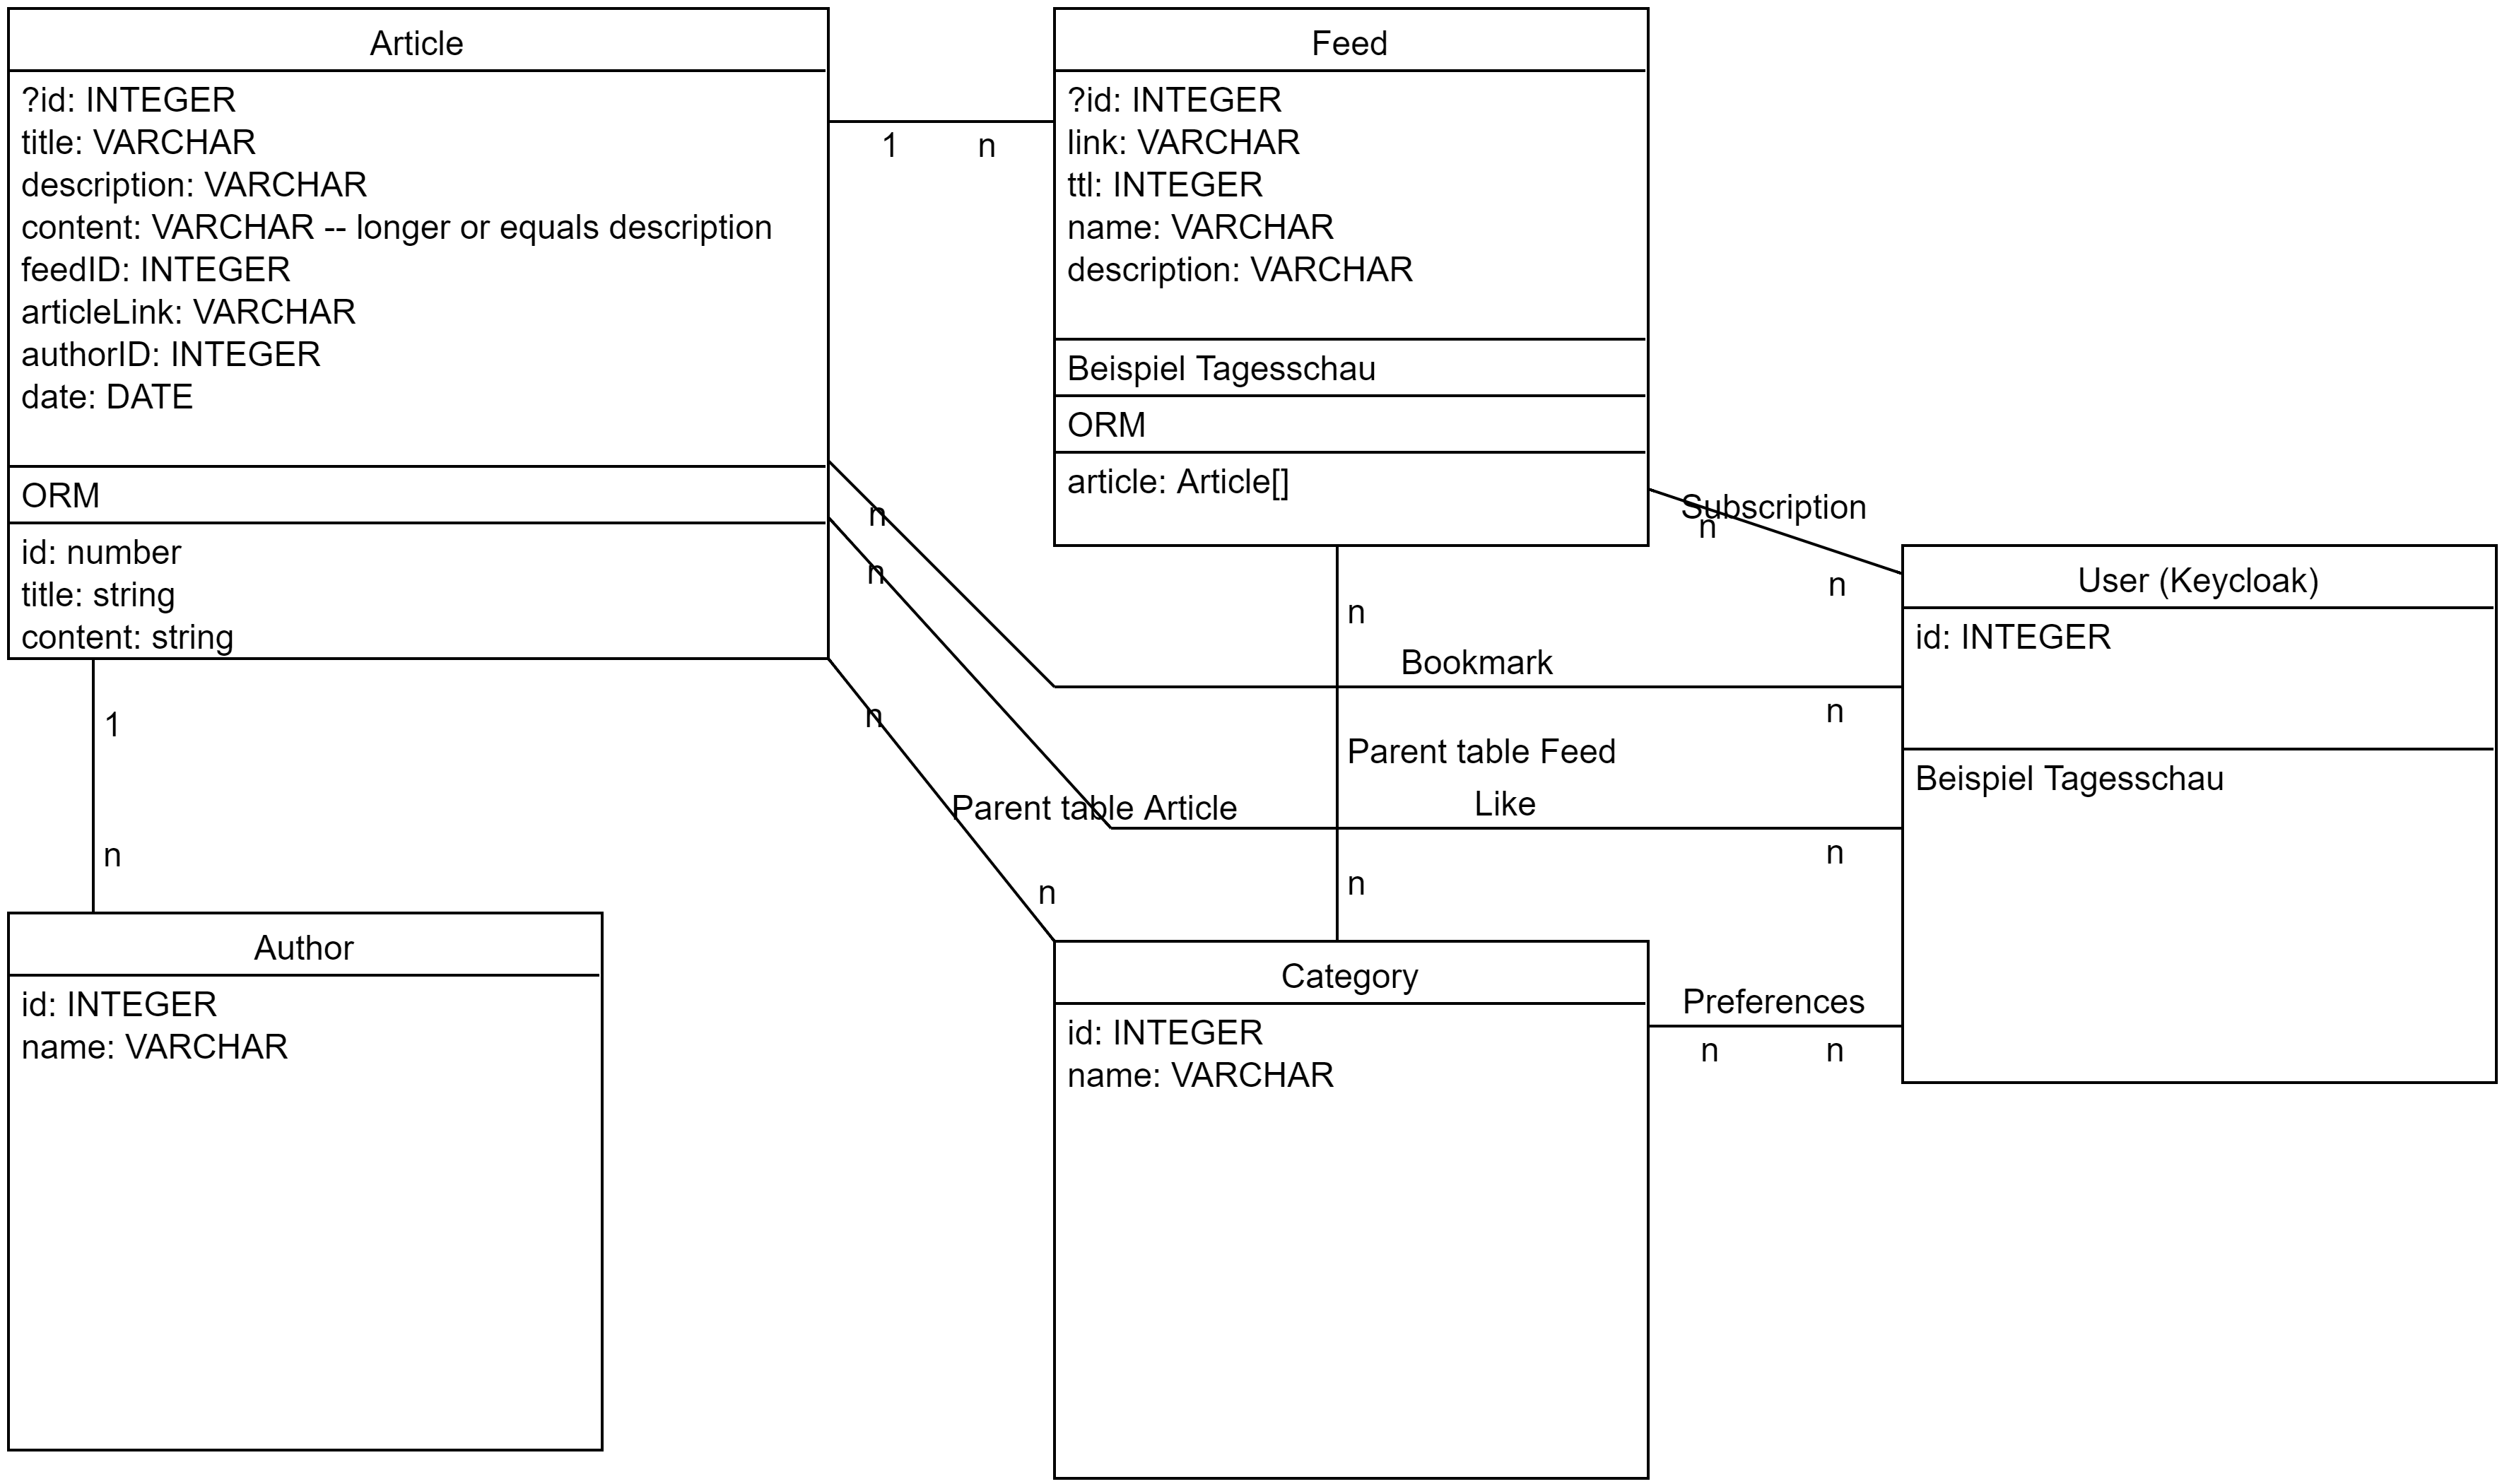
\includegraphics[width=\linewidth]{Database_Model.png}
    \caption{Datendefinition innerhalb der Datenbank}
    \label{fig:databaseORM}
\end{figure}
\end{quotation}
Bearbeitet von Jonas Eppard und Tim Horlacher.

\subsubsection{SKIOS-83 List of initial Feeds}
Das Ticket \enquote{SKIOS-83 List of initial Feeds} hatte folgende User Story:
\begin{quotation}
    As a developer I would like a list of initial feeds that we can poll before giving users the ability to add them in manually. 
    Goal of this story is to find 20-30 good (non reddit) feeds.\\
    \textbf{Acceptance Criteria}
    \begin{itemize}
        \item 20-30 feeds have been found and contain actual articles
        \item Structure of feeds is similar enough for polling service 
        \item The List is documented either in confluence or JSON in polling-service
    \end{itemize}
\end{quotation}
Bearbeitet von Theo Krinitz
Reviewed von Jannik Springer

\subsubsection{SKIOS-92 Initialize Keycloak}
Das Ticket \enquote{SKIOS-92 Initialize Keycloak} hatte folgende User Story:
\begin{quotation}
    As a developer I want to connect keycloak~\parencite{web/Keycloak} to our services and protect certain resources. \\
    \textbf{Acceptance Criteria}
    \begin{itemize}
        \item Two keycloak realms exist (production, testing)
        \item Our frontend connects to keycloak and resources are protectable
        \item Our backend connects to keycloak and resources are protectable
        \item Both realms have roles for users and admins
    \end{itemize}
\end{quotation}
Bearbeitet von Tim Horlacher.
Reviewed von Lukas Huida.

\subsubsection{SKIOS-93 Document Submission Guideline}
Das Ticket \enquote{SKIOS-93 Document Submission Guideline} hatte folgende User Story:
\begin{quotation}
    As a team member i would like to know what should be documented in our final documentation. \\
    \textbf{Acceptance Criteria}
    \begin{itemize}
        \item A confluence page should document what should be documented
    \end{itemize}
\end{quotation}
Bearbeitet von Tim Horlacher.
Reviewed von Amos Groß.

\subsubsection{SKIOS-74 Extend workflow to include wontfix}
Das Ticket \enquote{SKIOS-74 Extend workflow to include wontfix} hatte folgende User Story:
\begin{quotation}
    As a team member, I would like a wontfix state to disregard tickets.
    Goal of this story is to modify the current issue workflow used by jira.
    Note: this might require admin rights (contact PO or Architect for this) \\
    \textbf{Acceptance Criteria}
    \begin{itemize}
        \item Wontfix status exists
        \item The status contains the done property (is striked out)
    \end{itemize}
\end{quotation}
Bearbeitet von Lukas Huida.
Reviewed von Amos Groß.

\subsubsection{SKIOS-85 Repeated Polling runs}
Das Ticket \enquote{SKIOS-85 Repeated Polling runs} hatte folgende User Story:
\begin{quotation}
    As a developer I would like the polling service to be run as a cron job. \\
    \textbf{Acceptance Criteria}
    \begin{itemize}
        \item Polling service is called in Intervalls.
        \item Pod is not running all the time.
    \end{itemize}
\end{quotation}
Bearbeitet von Lukas Huida.
Reviewed von Tim Horlacher.

\subsubsection{SKIOS-63 Create Issue Template}
Das Ticket \enquote{SKIOS-63 Create Issue Template} hatte folgende User Story:
\begin{quotation}
    As a member of the Jira org, I would like to have a default template for issues. \\
\textbf{Acceptance Criteria}
\begin{itemize}
    \item An issue template exists for User Stories
\end{itemize}
\end{quotation}
Bearbeitet von Amos Groß.
Reviewed von Lukas Huida.

\subsubsection{SKIOS-77 Subscription Management Endpoints}
Das Ticket \enquote{SKIOS-77 Subscription Management Endpoints} hatte folgende User Story:
\begin{quotation}
    As a front end developer I would like endpoints for subscription management so that I can create its interface.
    Endpoint need to fulfill the following use cases:
    \begin{itemize}
        \item List subscribed feeds of current user
        \item Paginated fetch of most recent articles from all feeds
        \item Subscribe current user to feed
    \end{itemize}

    This functionality is part of the core-service \\
\textbf{Acceptance Criteria}
\begin{itemize}
    \item Use cases above can be performed with created endpoints
    \item Implementation contains reusable components for rest of plattform (aka is good code)
\end{itemize}
\end{quotation}
Bearbeitet von Amos Groß.
Reviewed von Tim Horlacher.

\subsubsection{SKIOS-106 ORM in Polling Service}
Das Ticket \enquote{SKIOS-106 ORM in Polling Service} hatte folgende User Story:
\begin{quotation}
    As a developer of our polling service I would like to use our shared ORM.
    Goal of this story is to replace all current ORM or datatbase logic with the new common node module and to load mock articles into the database following the structures provided.
\textbf{Acceptance Criteria}
\begin{itemize}
    \item Polling service now uses the common ORM logic
    \item Database is loaded up with min. of 5-10 Articles (using ORM)
\end{itemize}
\end{quotation}
Bearbeitet von Jannik Springer.
Reviewed von Lukas Huida.

\section{Sprint 3}

\subsection{Produktincrement}
\subsection{Charts}
\subsection{Probleme und Verbesserungen}

\subsection{Bearbeitete User Storys}
\subsubsection{SKIOS-116 Structure and table of contents for submission (\LaTeX)}
Das Ticket \enquote{SKIOS-116 Structure and table of contents for submission (\LaTeX)}
hatte folgende User Story:
\begin{quotation}
    As a team member, I would like to have a rough structure to orient myself while writing our submission documentation.\\
    For this story, please read the requirements and guidelines set out by Garidis and develop a rough idea on how to structure our \LaTeX project.\\
    \textbf{Acceptance Criteria}
    \begin{itemize}
        \item Table of contents is created (with \textbackslash{}section, \textbackslash{}subsection, etc.) in \LaTeX
        \item Structure reflects guidelines of Garidis
        \item Structure is explained in confluence page
        \item Existing \LaTeX~stories have a defined place where their pages will go
    \end{itemize}
\end{quotation}
Dies wurde folgendermaßen gelöst:
\begin{quotation}
    Es wurde die Struktur dieses \LaTeX-Dokuments angelegt. Hierbei musste nur das Inhaltsverzeichnis
    angelegt werden, da das \LaTeX-Template schon vorhanden war.
    Die Verwendung wurde in Confluence dokumentiert.
\end{quotation}
Bearbeitet von Jonas Eppard.

\subsubsection{Skios-79 Basic Article Endpoints}
Das Ticket \enquote{Skios-79 Basic Article Endpoints} hatte folgende User Story:
\begin{quotation}
    As a front-end developer I would like to have endpoints to base article views off of so that i can create their pages.\\
    \textbf{Acceptance Criteria}
    \begin{itemize}
        \item Endpoints are created to cover the case above including fieldresolver for 1-n and n-m relations
        \item This functionality is implemented in core-service
    \end{itemize}
\end{quotation}
Bearbeitet von Theo Krinitz
Reviewed von Jonas Eppard

\subsubsection{SKIOS-134 Fix core-service tests}
Das Ticket \enquote{SKIOS-134 Fix core-service tests} hatte folgende User Story:
\begin{quotation}
    As a developer I want a working testing framework, which implements unit and integration tests.\\
    \textbf{Acceptance Criteria}
    \begin{itemize}
        \item newman is installed inside dev container
        \item npm script is added that runs newman tests
    \end{itemize}
\end{quotation}
Bearbeitet von Theo Krinitz
Reviewed von Jannik Springer

\subsubsection{SKIOS-73 Place new logo in git, jira, confluence, etc}
Das Ticket \enquote{SKIOS-73 Place new logo in git, Jira, confluence, etc} hatte folgende User Story:
\begin{quotation}
    As a Product Owner I want our logo to be placed in the git repository, Jira \& confluence. \\
    \textbf{Requirements}
    \begin{itemize}
        \item Add branding for Skiosa
        \item Possibly also change look of Jira (at the top) and make it use our colorscheme.  
    \end{itemize}   
    
    \textbf{Acceptance Criteria}
    \begin{itemize}
        \item Skiosa Brandig is present in Git and Jira.
    \end{itemize}
\end{quotation}
Bearbeitet von Lukas Huida.
Reviewed von Jonas Eppard.

\subsubsection{SKIOS-76 Automatic Reviewer Suggestions}
Das Ticket \enquote{SKIOS-76 Automatic Reviewer Suggestions} hatte folgende User Story:
\begin{quotation}
    As a developer I want to have a way to automatically suggest reviewers for a PR. \\
    \textbf{Acceptance Criteria}
    \begin{itemize}
        \item Added Codeowners to every repo.
    \end{itemize}
\end{quotation}
Bearbeitet von Lukas Huida.
Reviewed von Tim Horlacher.

\subsubsection{SKIOS-91 Checklist for PRs}
Das Ticket \enquote{SKIOS-91 Checklist for PRs} hatte folgende User Story:
\begin{quotation}
    As a developer, I would like to have a reminder to check off the checklist from our contributing guidelines. \\
    \textbf{Acceptance Criteria}
    \begin{itemize}
        \item Every PR contains comment or default text including the checklist.
    \end{itemize}
\end{quotation}
Bearbeitet von Lukas Huida.
Reviewed von Jonas Eppard.

\subsubsection{SKIOS-111 Angular Design Boilerplate}
Das Ticket \enquote{SKIOS-111 Angular Design Boilerplate} hatte folgende User Story:
\begin{quotation}
    As a frontend developer I would like our frontend to have the basic components.
    Goal of this story ist to create components for:
    \begin{itemize}
        \item Buttons
        \item The Sidebar
        \item feeds
    \end{itemize}
\textbf{Acceptance Criteria}
\begin{itemize}
    \item Angular components are created for Buttons, Sidebar, Feeds
    \item The components are visibly identical to those in figma
    \item Button components can execute code when clicked on
    \item components should look according to current color mode (light / dark)
    \item Favicon of frontend is Skiosa Favicon
    \item Sidebar expands on mobile (see hamburger icon on pages like github, etc.)
\end{itemize}
\end{quotation}
Bearbeitet von Simon Morgenstern.
Reviewed von Lukas Huida.

\subsubsection{SKIOS-119 Frontend README}
Das Ticket \enquote{SKIOS-119 Frontend README} hatte folgende User Story:
\begin{quotation}
    As a developer, I would like a README in frontend service so that I read up on information on how to use it. \\
\textbf{Acceptance Criteria}
\begin{itemize}
    \item README is created
    \item README includes:
    \begin{itemize}
        \item development guide (how to start application, use devcontainer)
        \item description of service
        \item requirements for service
        \item service lead
    \end{itemize}
\end{itemize}
\end{quotation}
Bearbeitet von Lukas Huida.
Reviewed von Amos Groß.

\subsubsection{SKIOS-120 Deployment README}
Das Ticket \enquote{SKIOS-120 Deployment README} hatte folgende User Story:
\begin{quotation}
    As a developer, I would like a README in deployment so that I read up on information on how to use it. \\
\textbf{Acceptance Criteria}
\begin{itemize}
    \item README is created
    \item README includes:
    \begin{itemize}
        \item development guide (how to start application, use devcontainer)
        \item description of service
        \item requirements for service
        \item service lead
    \end{itemize}
\end{itemize}
\end{quotation}
Bearbeitet von Lukas Huida.
Reviewed von Amos Groß.

\subsubsection{SKIOS-137 Angular Service Framework}
Das Ticket \enquote{SKIOS-137 Angular Service Framework} hatte folgende User Story:
\begin{quotation}
    As a developer I would like to have angular services for our qraphql endpoints. \\
\textbf{Acceptance Criteria}
\begin{itemize}
    \item A library is found to automatically generate or facilitate graphql query creation
    \item Framework for creating graphql queries is created
    \item existing services are modified
    \item at minimum, one service is created to explain how to use this framework
\end{itemize}
\end{quotation}
Bearbeitet von Lukas Huida.
Reviewed von Amos Groß.

\subsubsection{SKIOS-138 Use Keycloak in GraphQL}
Das Ticket \enquote{SKIOS-138 Use Keycloak in GraphQL} hatte folgende User Story:
\begin{quotation}
    As a developer I want to secure some GraphQL resolver with our Keycloak. \\
    \textbf{Acceptance Criteria}
    \begin{itemize}
        \item Every resolver can be secured with Keycloak.
        \item An example resolver is created with Keycloak authentication.
    \end{itemize}
\end{quotation}
Bearbeitet von Lukas Huida.
Reviewed von Tim Horlacher.

\subsubsection{SKIOS-123 LaTeX Requirements Page}
Das Ticket \enquote{SKIOS-123 LaTeX Requirements Page} hatte folgende User Story:
\begin{quotation}
    As a team member I would like to have our requirements documented in confluence so that I won't fail this class. \\
\textbf{Acceptance Criteria}
\begin{itemize}
    \item A page is created in LaTeX
    \item Page includes:
    \begin{itemize}
        \item functional requirements
        \item non functional requirements 
        \item optional and mandatory
    \end{itemize}
    \item Has a table explaining changes made to these over the course of the project
\end{itemize}
\end{quotation}
Bearbeitet von Amos Groß.
Reviewed von Lukas Huida.

\subsubsection{SKIOS-133 ORM Readme}
Das Ticket \enquote{SKIOS-133 ORM Readme} hatte folgende User Story:
\begin{quotation}
    As a developer, I would like a README for ORM so that I read up on information on how to use it. \\
\textbf{Acceptance Criteria}
\begin{itemize}
    \item README is created
    \item README includes:
    \begin{itemize}
        \item development guide (how to create tags and to embed it to package.json)
        \item description of what this module does
        \item code owners 
    \end{itemize}
\end{itemize}
\end{quotation}
Bearbeitet von Jonas Eppard.
Reviewed von Lukas Huida.

\subsubsection{SKIOS-122 LaTeX Architecture Overview}
Das Ticket \enquote{SKIOS-122 LaTeX Architecture Overview} hatte folgende User Story:
\begin{quotation}
    As a team member I would like to have our architecture documented in confluence so that I won’t fail this class.
\textbf{Acceptance Criteria}
\begin{itemize}
    \item A page is created in our LaTeX documentation
    \item Services are listed and explained
    \item CI/CD infrasturture is explained
    \item Security Infrastructure (Keycloak)
    \item The Page explains the architecture in text form (prosa) 
    \item A diagram (not UML) is created to visualize our plattform architecture
\end{itemize}
\end{quotation}
Bearbeitet von Tim Horlacher und Lukas Huida.
Reviewed von Amos Groß.

\subsubsection{SKIOS-84 Initial Uniform Polling Implementation}
Das Ticket \enquote{SKIOS-84 Initial Uniform Polling Implementation} hatte folgende User Story:
\begin{quotation}
    As a developer I would like an initial implementaton of the polling service.\\
    This implementation should parse a single \enquote{type} of RSS feeds including at minimum the following:
    
    \begin{itemize}
        \item Link
        \item Titel
        \item Beschreibung
    \end{itemize}

    If an article doesn't contain this information it is ignored.\\
    If an article contains more information than this that information will also be ignored (will be parsed in later story)\\
    After parsing, it loads the information into the database. \\
\textbf{Acceptance Criteria}
\begin{itemize}
    \item Service can poll the structure above
    \item Polling service loads data into DB
    \item Multiple runs of the service don't produce duplicate data
\end{itemize}
\end{quotation}
Bearbeitet von Jannik Springer.
Reviewed von Lukas Huida.

\subsubsection{SKIOS-109 Backend Feed Mutation}
Das Ticket \enquote{SKIOS-109 Backend Feed Mutation} hatte folgende User Story:
\begin{quotation}
As a developer, I would like to have muations for creating and deleting feeds.
Goal of this story is to create Graphql Mutation to add a feed into our database. \\
\textbf{Acceptance Criteria}
\begin{itemize}
    \item Graphql mutation is created for feeds
    \item calling one of the mutations results in a feed being created in the database
    \item calling the mutation is possible only knowing the url of a feed (all other “not null” fields are left blank or filled with defaults)
    \item calling the other mutation (by ID) results in the specified feed being deleted
    \item deletion should only be possible for logged in users with a specific keycloak role
    \item creation should be possible for all logged in users
\end{itemize}
\end{quotation}
Bearbeitet von Marcel Alex und Tim Horlacher.
Reviewed von Lukas Huida.

\subsubsection{SKIOS-115 Core Service README}
Das Ticket \enquote{SKIOS-115 Core Service README} hatte folgende User Story:
\begin{quotation}
    As a developer, I would like a README in core service so that I read up on information on how to use it. \\
\textbf{Acceptance Criteria}
\begin{itemize}
    \item README is created
    \item README includes:
    \begin{itemize}
        \item development guide (how to start application, use devcontainer)
        \item description of what this module does
        \item requirements for service
        \item service lead
    \end{itemize}
\end{itemize}
\end{quotation}
Bearbeitet von Tim Horlacher
Reviewed von Jonas Eppard.

\subsubsection{SKIOS-117 Polling Service README}
Das Ticket \enquote{SKIOS-117 Polling Service README} hatte folgende User Story:
\begin{quotation}
    As a developer, I would like a README in polling service so that I read up on information on how to use it. \\
\textbf{Acceptance Criteria}
\begin{itemize}
    \item README is created
    \item README includes:
    \begin{itemize}
        \item development guide (how to start application, use devcontainer)
        \item description of service
        \item requirements for service
        \item service lead
    \end{itemize}
\end{itemize}
\end{quotation}
Bearbeitet von Jannik Springer.
Reviewed von Lukas Huida.

\subsubsection{SKIOS-121 PoC READMEs}
Das Ticket \enquote{SKIOS-121 PoC READMEs} hatte folgende User Story:
\begin{quotation}
    As a developer, I would like a README in all PoCs so that I read up on information on how to use it. \\
\textbf{Acceptance Criteria}
\begin{itemize}
    \item README is created
    \item README includes:
    \begin{itemize}
        \item development guide (how to start application, use devcontainer)
        \item goal of PoC
        \item link to Story of POC
        \item result of PoC
    \end{itemize}
\end{itemize}
\end{quotation}
Bearbeitet von Tim Horlacher
Reviewed von Amos Groß.

\subsubsection{SKIOS-124 \LaTeX Use cases page and UML}
Das Ticket \enquote{SKIOS-124 \LaTeX Use cases page and UML} hatte folgende User Story:
\begin{quotation}
    As a team member I would like to have our use cases documented in LaTeX so that I won't fail this class. \\
\textbf{Acceptance Criteria}
\begin{itemize}
    \item A page is created in LaTeX
    \item Page includes a use case diagram for:
    \begin{itemize}
        \item overview page
        \item settings page
        \item view page
    \end{itemize}
    \item The different use cases for SKIOSA are explained in text form (prosa) and embedd and explain the use case diagrams
    \item Page is spellchecked and contains no spelling mistakes (TEST THIS IN REVIEW)
    \item Text has been read by at least one other team member
\end{itemize}
\end{quotation}
Bearbeitet von Jonas Eppard und Sabrina Ladner.
Reviewed von Sabrina Ladner und Amos Groß.

\subsubsection{SKIOS-127 Finalize ORM}
Das Ticket \enquote{SKIOS-127 Finalize ORM} hatte folgende User Story:
\begin{quotation}
    As a developer, I would like to finalize our ORM, so that I can load data into the DB without having to fear it breaking.
\textbf{Acceptance Criteria}
\begin{itemize}
    \item Urls are Unique
    \item Articles have a timestamp
    \item Changes are signed off by both Architects
\end{itemize}
\end{quotation}
Bearbeitet von Jonas Eppard und Jannik Springer.
Reviewed von Tim Horlacher, Lukas Huida und Jannik Springer.

\subsubsection{SKIOS-82 Feed Overview Page}
Das Ticket \enquote{SKIOS-82 Feed Overview Page} hatte folgende User Story:
\begin{quotation}
    As a user of Skiosa, I would like to view a feed, so that I can decide if I want to subscribe to it.
    Content of this story is to implemented an overview page for feeds based on our mockups (this will exclude recommended feeds if part of the mockup). \\
\textbf{Acceptance Criteria}
\begin{itemize}
    \item The page displays: 
    \begin{itemize}
        \item name
        \item description
        \item articles
    \end{itemize}
    \item Page is designed as specified in figma
    \item The subscribe button subscribes a user (if not logged in redirects to login page)
\end{itemize}
\end{quotation}
Bearbeitet von Marcel Alex.
Reviewed von Lukas Huida.

\subsubsection{SKIOS-80 Article View Page}
Das Ticket \enquote{SKIOS-80 Article View Page} hatte folgende User Story:
\begin{quotation}
    As a user of Skiosa, I would like to view an article.
    Content of this story is to implemented the view page based on our mockups without its references to other articles or likes/bookmarks. \\
\textbf{Acceptance Criteria}
\begin{itemize}
    \item Title, link, description, etc. are displayed 
    \item Page uses endpoints from core-sevice to achieve this
\end{itemize}
\end{quotation}
Bearbeitet von Simong Morgenstern und Jonas Eppard.
Reviewed von Lukas Huida.

\subsubsection{SKIOS-78 Subscription Page}
Das Ticket \enquote{SKIOS-78 Subscription Page} hatte folgende User Story:
\begin{quotation}
    As a user of Skiosa I would like to have a page for my subscriptions so that I can use them.
    Goal of this story is to use the backend components provided in SKIOS-77 and to create a subscription page following our design.
    Note: Subscription indicator of mockup will not be in scope for this story. \\
\textbf{Acceptance Criteria}
\begin{itemize}
    \item Subcription page follows design of figma mockups
    \item Page contains list of the current users subscriptions
    \item For non logged in users, this page redirects to login
\end{itemize}
\end{quotation}
Bearbeitet von Amos Groß.
Reviewed von Lukas Huida.

\subsubsection{SKIOS-94 Overview Page}
Das Ticket \enquote{SKIOS-94 Overview Page} hatte folgende User Story:
\begin{quotation}
    As a user I would like to have a homepage.
    Goal of this story is to use the endpoints of the preliminary recomendation service and to display them as seen in the mockup.
    The recomended feeds are not to be regarded here. \\
\textbf{Acceptance Criteria}
\begin{itemize}
    \item Overview Page exists at root ('/')
    \item Overview Page follows design scheme 
\end{itemize}
\end{quotation}
Bearbeitet von Amos Groß.
Reviewed von Simon Morgenstern.

\subsubsection{SKIOS-114 Roadmap in Confluence}
Das Ticket \enquote{SKIOS-114 Roadmap in Confluence} hatte folgende User Story:
\begin{quotation}
    As a Product owner I would like a roadmap in confluence. \\
\textbf{Acceptance Criteria}
\begin{itemize}
    \item Preliminary Roadmap in Front Page of Confluence is Replaced
    \item Roadmap reflects or PIs
\end{itemize}
\end{quotation}
Bearbeitet von Amos Groß.
Reviewed von Lukas Huida.

\subsubsection{SKIOS-123 Latex Requirements Page}
Das Ticket \enquote{SKIOS-123 Latex Requirements Page} hatte folgende User Story:
\begin{quotation}
    As a team member I would like to have our requirements documented in confluence so that I won't fail this class. \\
\textbf{Acceptance Criteria}
\begin{itemize}
    \item A page is created in LaTeX
    \item Has a table explaining changes made to these over the course of the project
    \item Page includes:
    \begin{itemize}
    \item functional requirements
    \item non functional requirements 
    \item optional and mandatory
    \end{itemize}
\end{itemize}
\end{quotation}
Bearbeitet von Amos Groß.
Reviewed von Lukas Huida.

\subsubsection{SKIOS-113 LaTeX Organigram/Orthography}
Das Ticket \enquote{SKIOS-113 LaTeX Organigram/Orthography} hatte folgende User Story:
\begin{quotation}
    As a team member I would like to have our orthography documented in confluence in LaTeX. \\
\textbf{Acceptance Criteria}
\begin{itemize}
    \item A page is created in LaTeX
    \item Page includes Diagram displaying team members
    \item Page includes short explanations for the jobs that the following roles undertook (even when in overlap with SCRUM)
    \begin{itemize}
        \item Service Lead
        \item Architects
        \item Product owner
        \item Scrum Master
        \item Team Member (optional)
    \end{itemize}
    \item Page is written in text form (prosa) and refers to diagram/organigramm
    \item Page explains WHY we chose to structure our team in this manner   
\end{itemize}
\end{quotation}
Bearbeitet von Theo Krinitz
Reviewed von Jannik Springer

\section{Sprint 4}
\subsection{Produktincrement}
\subsection{Charts}
\subsection{Probleme und Verbesserungen}

\subsection{Bearbeitete User Storys}
\subsubsection{SKIOS-145 Mutators and Resolvers for Bookmarks}
Das Ticket \enquote{SKIOS-145 Mutators and Resolvers for Bookmarks} hatte folgende User Story:
\begin{quotation}
    As a frontend developer I would like resolvers for bookmarks to be able to create and manage bookmarks. \\
\textbf{Acceptance Criteria}
\begin{itemize}
    \item A resolver is created for:
    \begin{itemize}
        \item Paginated fetch of all bookmarks
        \item Check if article is bookmarked (in article resolver!)
    \end{itemize}
    \item A mutation is created for:
    \begin{itemize}
        \item Adding bookmarks
        \item Removing Bookmarks
    \end{itemize}
\end{itemize}
\end{quotation}
Bearbeitet von Lukas Huida und Tim Horlacher.
Reviewed von Jonas Eppard.

\subsubsection{SKIOS-147 Angular Bookmarks Page}
Das Ticket \enquote{SKIOS-147 Angular Bookmarks Page} hatte folgende User Story:
\begin{quotation}
    As a user I would like to have a page to view my bookmarks in. \\
\textbf{Acceptance Criteria}
\begin{itemize}
    \item Page is created
    \item Button in sidebar is created and links to this page
    \item Page displays Bookmarks of User as specified in mockup
    \item Search and Filter Icons that exist in the mockup aren't shown in the angular page
\end{itemize}
\end{quotation}
Bearbeitet von Lukas Huida.
Reviewed von Simon Morgenstern.

\subsubsection{SKIOS-144 Mutators and Resolvers for Likes}
Das Ticket \enquote{SKIOS-144 Mutators and Resolvers for Likes} hatte folgende User Story:
\begin{quotation}
    As a frontend developer I would like resolvers for likes to be able to create and manage likes. \\
\textbf{Acceptance Criteria}
\begin{itemize}
    \item A resolver is created for:
    \begin{itemize}
        \item Check if article is in likes of user (in article resolver!)
    \end{itemize}
    \item A mutation is created for:
    \begin{itemize}
        \item Liking article
        \item Removing Like
    \end{itemize}
\end{itemize}
\end{quotation}
Bearbeitet von Tim Horlacher
Reviewed von Lukas Huida.

\subsubsection{SKIOS-164 LaTeX Meeting Summary}
Das Ticket \enquote{SKIOS-164 LaTeX Meeting Summary} hatte folgende User Story:
\begin{quotation}
    As a team member I would like a LaTeX page explaining the various meetings we organised in our project.
    This story will fill out section 2.3 \enquote{Zusammenarbeit} and If considered a bad title should be renamed to something containing the work \enquote{meetings}.
\textbf{Acceptance Criteria}
\begin{itemize}
    \item Page is created in LaTeX
    \item Page is Spell Checked in Review
    \item Page explains the following meetings:
    \begin{itemize}
        \item Estimations
        \item Bi Weeklys
        \item Dailys
        \item Planning
        \item Retro
        \item Review
        \item Roadmap Meetings (Held between PO and Tech Leads)
    \end{itemize}
    \item Explanations include:
    \begin{itemize}
        \item Frequency of the meeting (once a week, every sprint, every class, alternating such as with estimations etc.)
        \item Purpose of the meeting (why do we need this meeting?)
        \item Structure of the meeting (ex. bi weekly = daily, then general talking points and discussion)
        \item Result of the meeting (ex. Retro = Action items)
        \item If present team specifc adaptations to these meetings (ex. Daily being held once a week)
    \end{itemize}
    \item All explanations conform with SCRUM (see \url{https://scrumguides.org/docs/scrumguide/v2020/2020-Scrum-Guide-US.pdf#zoom=100})
    \item Individual Meetings are not explained in this section
\end{itemize}
\end{quotation}
Bearbeitet von Jannik Springer und Amos Groß.
Jeweils gegenseitig reviewed von Amos Groß und Jannik Springer.

\subsubsection{SKIOS-166 \LaTeX Technical Changelog}
Das Ticket \enquote{SKIOS-166 \LaTeX Technical Changelog} hatte folgende User Story:
\begin{quotation}
    As a team member, I would like changes to the technical understanding of our project to be documented.
    Goal of this story is to explain how our requirements regarding RSS, etc. changed throughout the project changed our requirements. \\
    This story will complete section 5.3 “Technische Änderungen zur anfänglichen Struktur”. \\
    Initial Requirements are not documented here (this is done in chapter 1).
\textbf{Acceptance Criteria}
\begin{itemize}
    \item Page is created in LaTeX
    \item Page is Spell Checked in Review
    \item Page lists changes to our technical understanding of the project:
    \begin{itemize}
        \item How RSS feeds work
        \item nessessity of a Recomendation Service
    \end{itemize}
    \item Page Explains changes to our requirements due to these changes
    \begin{itemize}
        \item Removing a creator page (due to lack of settings, ex. ttl)
    \end{itemize}
\end{itemize}
\end{quotation}
Bearbeitet von Tim Horlacher.
Reviewed von Amos Groß.


\subsubsection{SKIOS-151 Latex Roadmap Chapter}
Das Ticket \enquote{SKIOS-151 Latex Roadmap Chapter} hatte folgende User Story:
\begin{quotation}
    As a member of this team I would like to have a road map chapter, so that I won't fail this class.
    Note: this story should be done by the PO \\
\textbf{Acceptance Criteria}
\begin{itemize}
    \item LaTeX Chapter is created and filled out
    \item Chapter explains PIs
    \item Chapter explains Rationale behind Planning
\end{itemize}
\end{quotation}
Bearbeitet von Amos Groß
Reviewed von Jonas Eppard.

\subsubsection{SKIOS-153 LaTeX Mockup showcase}
Das Ticket \enquote{SKIOS-153 LaTeX Mockup showcase} hatte folgende User Story:
\begin{quotation}
    As a team member I would like to have a page explaining our Mockups. \\
\textbf{Acceptance Criteria}
\begin{itemize}
    \item Page is is created in LaTeX
    \item Page is spellchecked
    \item Page explains our Design Language
    \begin{itemize}
        \item What a design language is (quick definition)
        \item What our design language is
        \item What our colorscheme is
    \end{itemize}
    \item Page explains our usage of Figma
    \begin{itemize}
        \item Common Components
        \item Common Colors (figma styles)
    \end{itemize}
    \item Page showcases every page of our figma designs
    \begin{itemize}
        \item Includes Screenshot
        \item Includes Quick summary (2 sentences on the behaviour of the page and what it shows, ex. clicking on subscribe in feed overview subscribes a user) 
        \item Focus on Actions that are not explained in use case ( section 1.4)
    \end{itemize}
\end{itemize}
\end{quotation}
Bearbeitet von Theo Krinitz
Reviewed von Amos Groß

